\documentclass{standalone}
\usepackage{tikz}
\usetikzlibrary{patterns, positioning}

\begin{document}
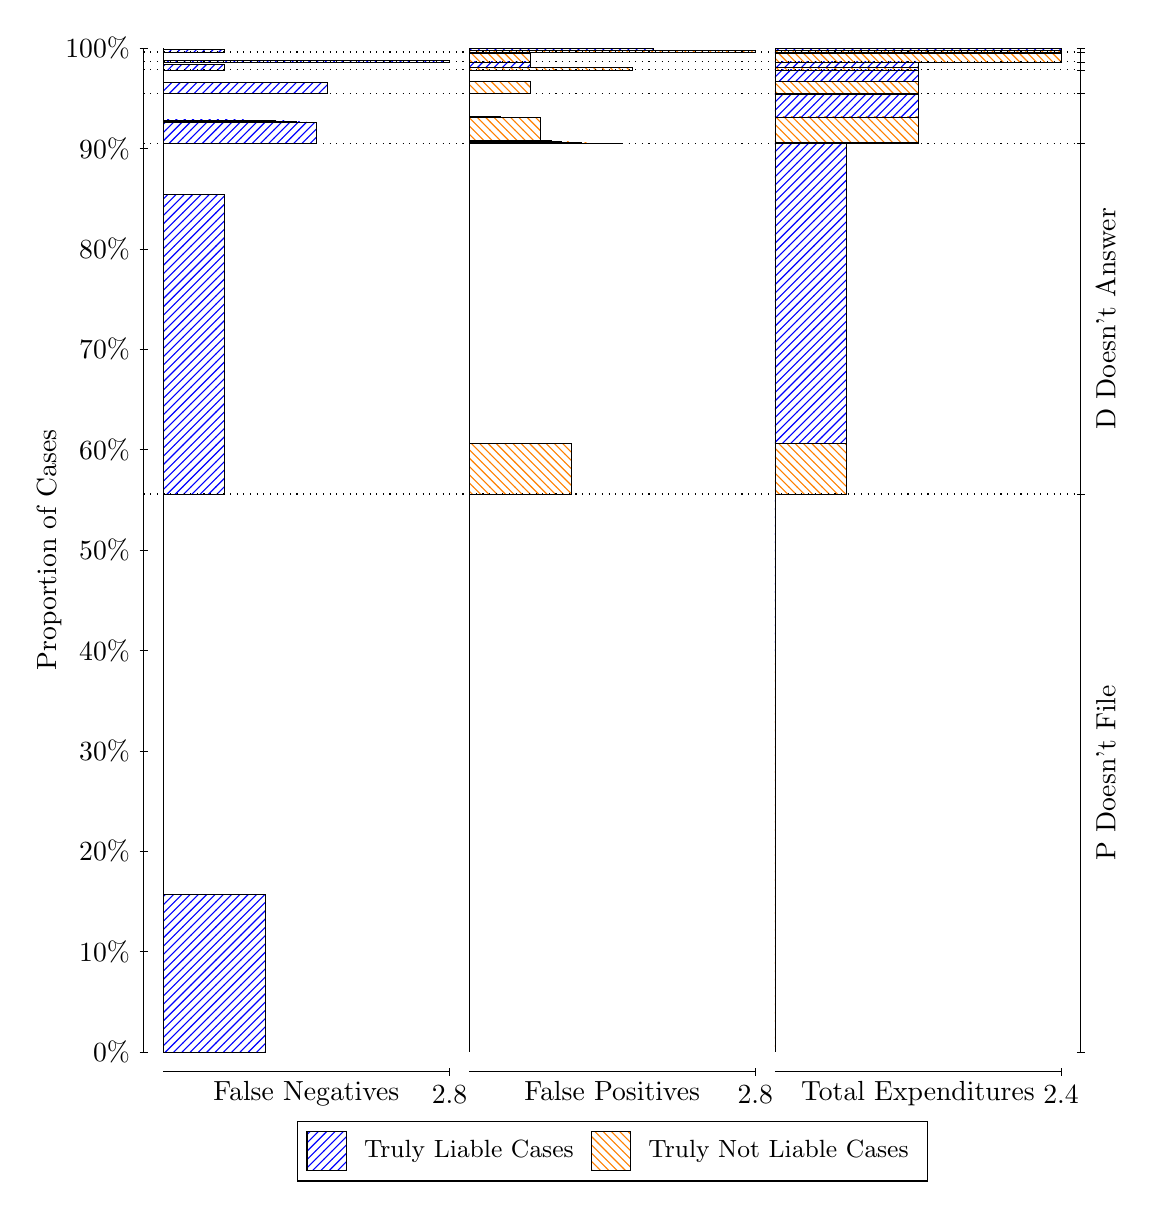
\begin{tikzpicture}
\draw[black, very thin] (1.5,1.75) -- (1.5,14.5);
\node[rotate=90, anchor=center] at (0.3, 8.125) {Proportion of Cases};
\draw[black, very thin] (1.45,1.75) -- (1.55,1.75);
\node[anchor=east] at (1.45, 1.75) {0\%};
\draw[black, very thin] (1.45,3.025) -- (1.55,3.025);
\node[anchor=east] at (1.45, 3.025) {10\%};
\draw[black, very thin] (1.45,4.3) -- (1.55,4.3);
\node[anchor=east] at (1.45, 4.3) {20\%};
\draw[black, very thin] (1.45,5.575) -- (1.55,5.575);
\node[anchor=east] at (1.45, 5.575) {30\%};
\draw[black, very thin] (1.45,6.85) -- (1.55,6.85);
\node[anchor=east] at (1.45, 6.85) {40\%};
\draw[black, very thin] (1.45,8.125) -- (1.55,8.125);
\node[anchor=east] at (1.45, 8.125) {50\%};
\draw[black, very thin] (1.45,9.4) -- (1.55,9.4);
\node[anchor=east] at (1.45, 9.4) {60\%};
\draw[black, very thin] (1.45,10.675) -- (1.55,10.675);
\node[anchor=east] at (1.45, 10.675) {70\%};
\draw[black, very thin] (1.45,11.95) -- (1.55,11.95);
\node[anchor=east] at (1.45, 11.95) {80\%};
\draw[black, very thin] (1.45,13.225) -- (1.55,13.225);
\node[anchor=east] at (1.45, 13.225) {90\%};
\draw[black, very thin] (1.45,14.5) -- (1.55,14.5);
\node[anchor=east] at (1.45, 14.5) {100\%};

\draw[black, very thin] (13.4,1.75) -- (13.4,14.5);
\draw[black, very thin] (13.35,1.75) -- (13.45,1.75);
\node[anchor=west] at (13.35, 1.75) {};
\draw[black, very thin] (13.35,8.8358) -- (13.45,8.8358);
\node[anchor=west] at (13.35, 8.8358) {};
\draw[black, very thin] (13.35,13.286) -- (13.45,13.286);
\node[anchor=west] at (13.35, 13.286) {};
\draw[black, very thin] (13.35,13.924) -- (13.45,13.924);
\node[anchor=west] at (13.35, 13.924) {};
\draw[black, very thin] (13.35,14.223) -- (13.45,14.223);
\node[anchor=west] at (13.35, 14.223) {};
\draw[black, very thin] (13.35,14.325) -- (13.45,14.325);
\node[anchor=west] at (13.35, 14.325) {};
\draw[black, very thin] (13.35,14.449) -- (13.45,14.449);
\node[anchor=west] at (13.35, 14.449) {};
\draw[black, very thin] (13.35,14.5) -- (13.45,14.5);
\node[anchor=west] at (13.35, 14.5) {};

\draw[black, very thin, pattern color=blue, pattern=north east lines] (1.75,1.75) rectangle (3.0476,3.754);
\draw[black, very thin, pattern color=orange, pattern=north west lines] (1.75,3.754) rectangle (1.75,8.8358);
\draw[black, very thin, pattern color=blue, pattern=north east lines] (1.75,8.8358) rectangle (2.5286,12.641);
\draw[black, very thin, pattern color=orange, pattern=north west lines] (1.75,12.641) rectangle (1.75,13.286);
\draw[black, very thin, pattern color=blue, pattern=north east lines] (1.75,13.286) rectangle (3.6964,13.555);
\draw[black, very thin, pattern color=blue, pattern=north east lines] (1.75,13.555) rectangle (3.5667,13.562);
\draw[black, very thin, pattern color=blue, pattern=north east lines] (1.75,13.562) rectangle (3.4369,13.568);
\draw[black, very thin, pattern color=blue, pattern=north east lines] (1.75,13.568) rectangle (3.3071,13.574);
\draw[black, very thin, pattern color=blue, pattern=north east lines] (1.75,13.574) rectangle (3.1774,13.58);
\draw[black, very thin, pattern color=blue, pattern=north east lines] (1.75,13.58) rectangle (3.0476,13.583);
\draw[black, very thin, pattern color=blue, pattern=north east lines] (1.75,13.583) rectangle (2.9179,13.585);
\draw[black, very thin, pattern color=blue, pattern=north east lines] (1.75,13.585) rectangle (2.7881,13.587);
\draw[black, very thin, pattern color=blue, pattern=north east lines] (1.75,13.587) rectangle (2.6583,13.588);
\draw[black, very thin, pattern color=orange, pattern=north west lines] (1.75,13.588) rectangle (1.75,13.924);
\draw[black, very thin, pattern color=blue, pattern=north east lines] (1.75,13.924) rectangle (3.8262,14.067);
\draw[black, very thin, pattern color=orange, pattern=north west lines] (1.75,14.067) rectangle (1.75,14.223);
\draw[black, very thin, pattern color=blue, pattern=north east lines] (1.75,14.223) rectangle (2.5286,14.293);
\draw[black, very thin, pattern color=orange, pattern=north west lines] (1.75,14.293) rectangle (1.75,14.325);
\draw[black, very thin, pattern color=blue, pattern=north east lines] (1.75,14.325) rectangle (5.3833,14.345);
\draw[black, very thin, pattern color=orange, pattern=north west lines] (1.75,14.345) rectangle (1.75,14.449);
\draw[black, very thin, pattern color=blue, pattern=north east lines] (1.75,14.449) rectangle (2.5286,14.48);
\draw[black, very thin, pattern color=orange, pattern=north west lines] (1.75,14.48) rectangle (1.75,14.5);
\draw[black, very thin, pattern color=orange, pattern=north west lines] (5.6333,1.75) rectangle (5.6333,6.8318);
\draw[black, very thin, pattern color=blue, pattern=north east lines] (5.6333,6.8318) rectangle (5.6333,8.8358);
\draw[black, very thin, pattern color=orange, pattern=north west lines] (5.6333,8.8358) rectangle (6.931,9.4813);
\draw[black, very thin, pattern color=blue, pattern=north east lines] (5.6333,9.4813) rectangle (5.6333,13.286);
\draw[black, very thin, pattern color=orange, pattern=north west lines] (5.6333,13.286) rectangle (7.5798,13.287);
\draw[black, very thin, pattern color=orange, pattern=north west lines] (5.6333,13.287) rectangle (7.45,13.289);
\draw[black, very thin, pattern color=orange, pattern=north west lines] (5.6333,13.289) rectangle (7.3202,13.291);
\draw[black, very thin, pattern color=orange, pattern=north west lines] (5.6333,13.291) rectangle (7.1905,13.294);
\draw[black, very thin, pattern color=orange, pattern=north west lines] (5.6333,13.294) rectangle (7.0607,13.302);
\draw[black, very thin, pattern color=orange, pattern=north west lines] (5.6333,13.302) rectangle (6.931,13.308);
\draw[black, very thin, pattern color=orange, pattern=north west lines] (5.6333,13.308) rectangle (6.8012,13.317);
\draw[black, very thin, pattern color=orange, pattern=north west lines] (5.6333,13.317) rectangle (6.6714,13.329);
\draw[black, very thin, pattern color=orange, pattern=north west lines] (5.6333,13.329) rectangle (6.5417,13.622);
\draw[black, very thin, pattern color=blue, pattern=north east lines] (5.6333,13.622) rectangle (6.2821,13.623);
\draw[black, very thin, pattern color=blue, pattern=north east lines] (5.6333,13.623) rectangle (6.1524,13.624);
\draw[black, very thin, pattern color=blue, pattern=north east lines] (5.6333,13.624) rectangle (6.0226,13.627);
\draw[black, very thin, pattern color=blue, pattern=north east lines] (5.6333,13.627) rectangle (5.8929,13.629);
\draw[black, very thin, pattern color=blue, pattern=north east lines] (5.6333,13.629) rectangle (5.7631,13.636);
\draw[black, very thin, pattern color=blue, pattern=north east lines] (5.6333,13.636) rectangle (5.6333,13.924);
\draw[black, very thin, pattern color=orange, pattern=north west lines] (5.6333,13.924) rectangle (6.4119,14.08);
\draw[black, very thin, pattern color=blue, pattern=north east lines] (5.6333,14.08) rectangle (5.6333,14.223);
\draw[black, very thin, pattern color=orange, pattern=north west lines] (5.6333,14.223) rectangle (7.7095,14.255);
\draw[black, very thin, pattern color=blue, pattern=north east lines] (5.6333,14.255) rectangle (6.4119,14.325);
\draw[black, very thin, pattern color=orange, pattern=north west lines] (5.6333,14.325) rectangle (6.4119,14.429);
\draw[black, very thin, pattern color=blue, pattern=north east lines] (5.6333,14.429) rectangle (5.6333,14.449);
\draw[black, very thin, pattern color=orange, pattern=north west lines] (5.6333,14.449) rectangle (9.2667,14.469);
\draw[black, very thin, pattern color=blue, pattern=north east lines] (5.6333,14.469) rectangle (7.969,14.5);
\draw[black, very thin, pattern color=orange, pattern=north west lines] (9.5167,1.75) rectangle (9.5167,6.8318);
\draw[black, very thin, pattern color=blue, pattern=north east lines] (9.5167,6.8318) rectangle (9.5167,8.8358);
\draw[black, very thin, pattern color=orange, pattern=north west lines] (9.5167,8.8358) rectangle (10.425,9.4813);
\draw[black, very thin, pattern color=blue, pattern=north east lines] (9.5167,9.4813) rectangle (10.425,13.286);
\draw[black, very thin, pattern color=orange, pattern=north west lines] (9.5167,13.286) rectangle (11.333,13.294);
\draw[black, very thin, pattern color=blue, pattern=north east lines] (9.5167,13.294) rectangle (11.333,13.301);
\draw[black, very thin, pattern color=orange, pattern=north west lines] (9.5167,13.301) rectangle (11.333,13.625);
\draw[black, very thin, pattern color=blue, pattern=north east lines] (9.5167,13.625) rectangle (11.333,13.915);
\draw[black, very thin, pattern color=orange, pattern=north west lines] (9.5167,13.915) rectangle (11.333,13.919);
\draw[black, very thin, pattern color=blue, pattern=north east lines] (9.5167,13.919) rectangle (11.333,13.924);
\draw[black, very thin, pattern color=orange, pattern=north west lines] (9.5167,13.924) rectangle (11.333,14.08);
\draw[black, very thin, pattern color=blue, pattern=north east lines] (9.5167,14.08) rectangle (11.333,14.223);
\draw[black, very thin, pattern color=orange, pattern=north west lines] (9.5167,14.223) rectangle (11.333,14.255);
\draw[black, very thin, pattern color=blue, pattern=north east lines] (9.5167,14.255) rectangle (11.333,14.325);
\draw[black, very thin, pattern color=orange, pattern=north west lines] (9.5167,14.325) rectangle (13.15,14.429);
\draw[black, very thin, pattern color=blue, pattern=north east lines] (9.5167,14.429) rectangle (13.15,14.449);
\draw[black, very thin, pattern color=orange, pattern=north west lines] (9.5167,14.449) rectangle (13.15,14.469);
\draw[black, very thin, pattern color=blue, pattern=north east lines] (9.5167,14.469) rectangle (13.15,14.5);
\draw[black, dotted] (1.5,8.8358) -- (13.4,8.8358);
\draw[black, dotted] (1.5,13.286) -- (13.4,13.286);
\draw[black, dotted] (1.5,13.924) -- (13.4,13.924);
\draw[black, dotted] (1.5,14.223) -- (13.4,14.223);
\draw[black, dotted] (1.5,14.325) -- (13.4,14.325);
\draw[black, dotted] (1.5,14.449) -- (13.4,14.449);
\draw[black, very thin] (1.75,1.5) -- (5.3833,1.5);
\node[anchor=north] at (3.5667, 1.5) {False Negatives};
\draw[black, very thin] (5.3833,1.45) -- (5.3833,1.55);
\node[anchor=north] at (5.3833, 1.45) {2.8};

\draw[black, very thin] (5.6333,1.5) -- (9.2667,1.5);
\node[anchor=north] at (7.45, 1.5) {False Positives};
\draw[black, very thin] (9.2667,1.45) -- (9.2667,1.55);
\node[anchor=north] at (9.2667, 1.45) {2.8};

\draw[black, very thin] (9.5167,1.5) -- (13.15,1.5);
\node[anchor=north] at (11.333, 1.5) {Total Expenditures};
\draw[black, very thin] (13.15,1.45) -- (13.15,1.55);
\node[anchor=north] at (13.15, 1.45) {2.4};

\node[black, centered, rotate=90] at (13.72, 5.2929) {P Doesn't File};
\node[black, centered, rotate=90] at (13.72, 11.061) {D Doesn't Answer};






\draw (7.449999999999999,1.5) node[draw=none] (baseCoordinate) {};
\begin{scope}[align=center]
        \matrix[scale=0.5, draw=black, below=0.5cm of baseCoordinate, nodes={draw}, column sep=0.1cm]{
            \node[rectangle, draw, minimum width=0.5cm, minimum height=0.5cm, pattern=north east lines, pattern color=blue] {}; &
            \node[draw=none, font=\small] (B) {Truly Liable Cases}; &
            \node[rectangle, draw, minimum width=0.5cm, minimum height=0.5cm, pattern=north west lines, pattern color=orange] {}; &
            \node[draw=none, font=\small] (B) {Truly Not Liable Cases}; \\
            };
\end{scope}

\end{tikzpicture}
\end{document}